\section{Resultate}

In unserem Schlussresultat ist die Superposition gut erkennbar. Ausgangsbild war eine Spirale auf der sich einige Punkte befinden mit der gleichen Stromst�rke. Pro Bild f�hrten wir 180\,000 Iterationen durch.

\newlength\breite
\setlength\breite{8cm}

\begin{figure}
		\centering
	\begin{tabular}{cc}
		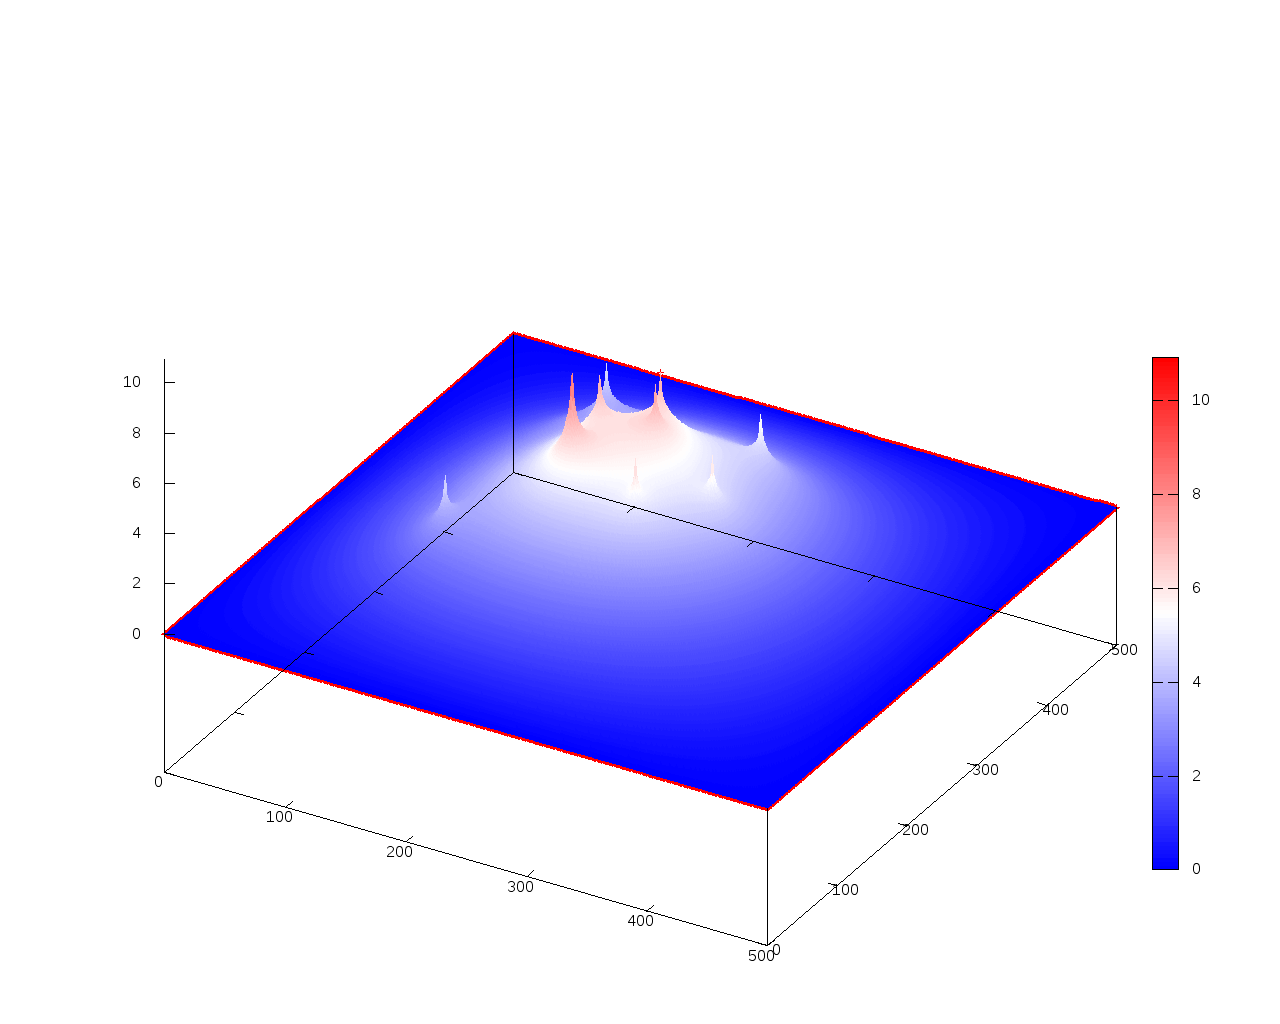
\includegraphics[width=\breite]{./images/resultate/step0111.png}
		& 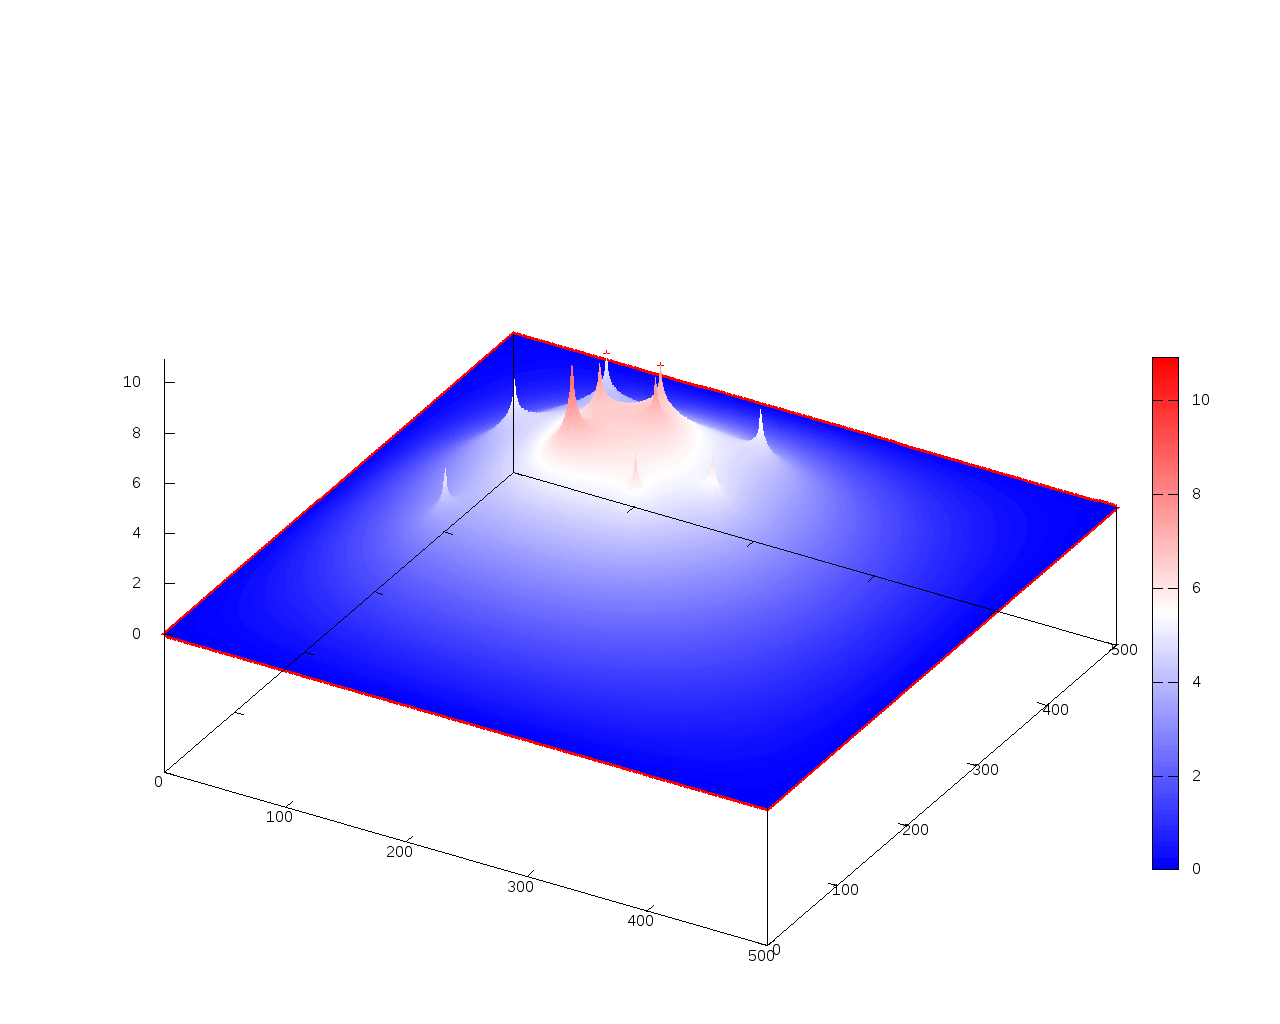
\includegraphics[width=\breite]{./images/resultate/step0112.png}\\
		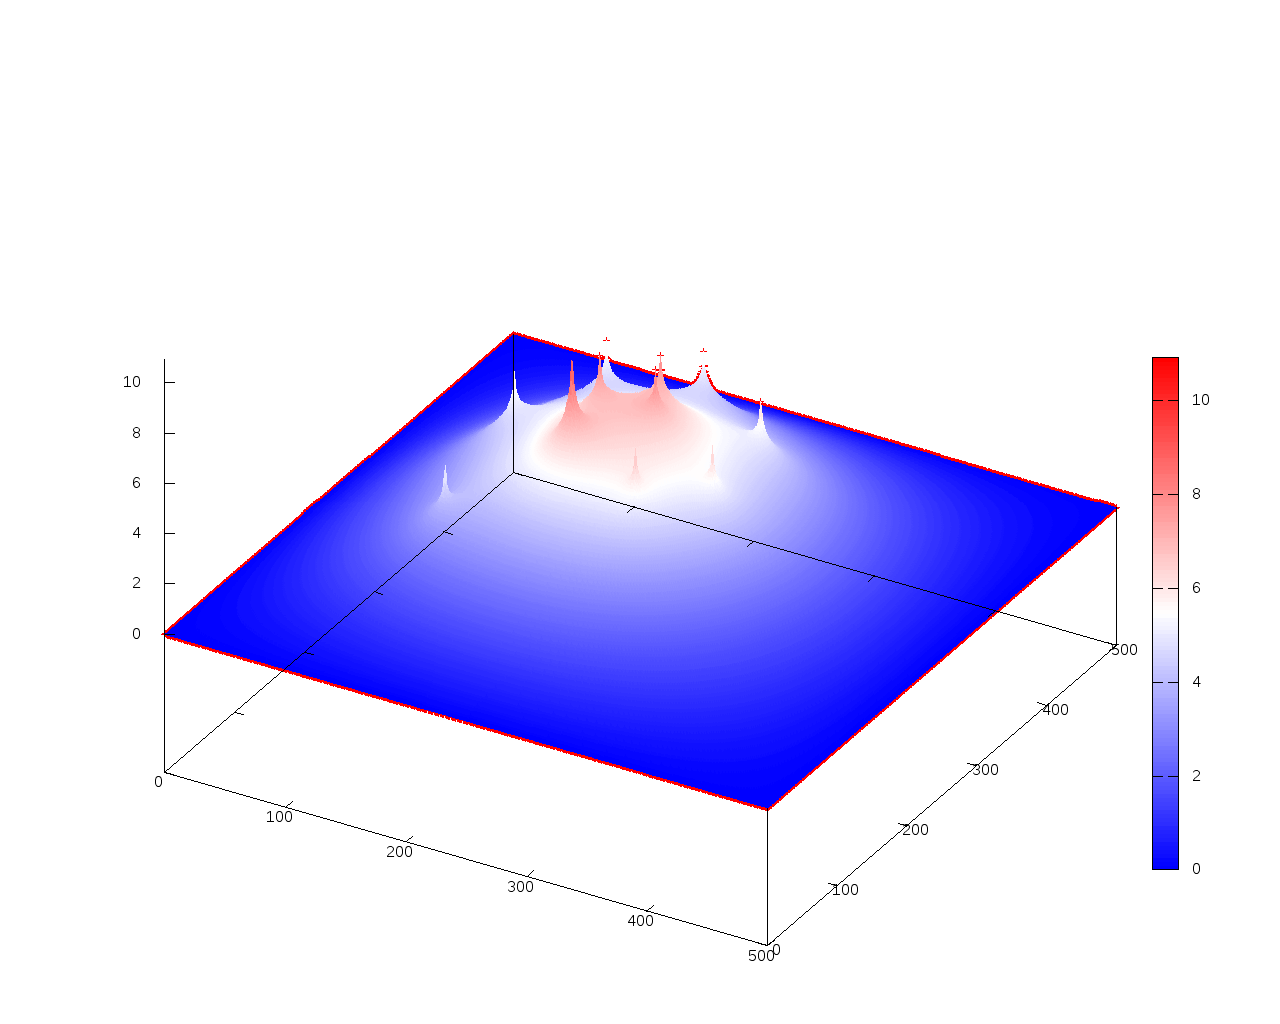
\includegraphics[width=\breite]{./images/resultate/step0113.png}
		& 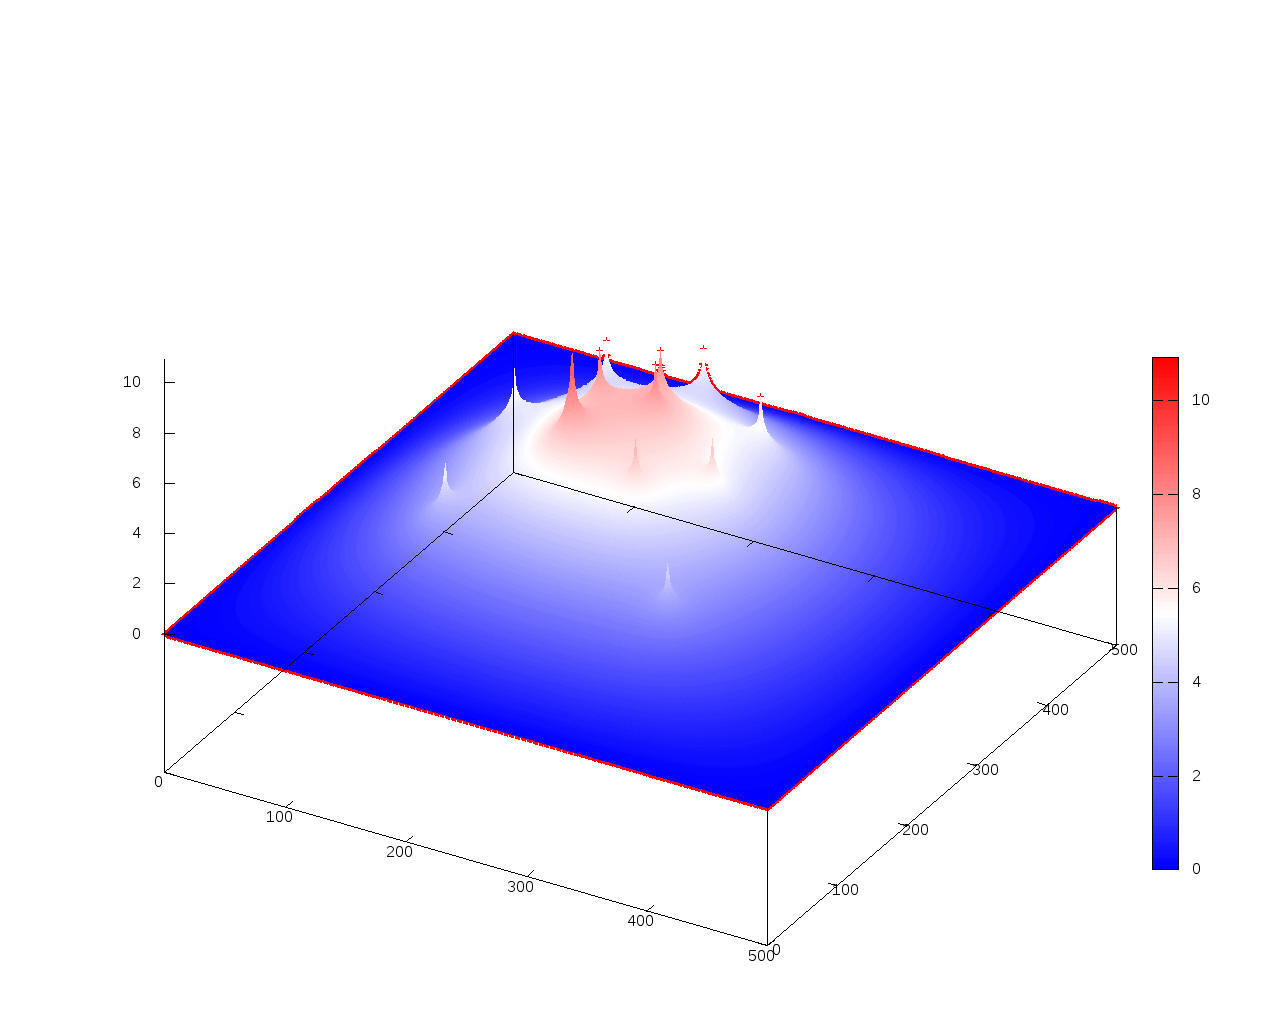
\includegraphics[width=\breite]{./images/resultate/step0138.png}
	\end{tabular}		
		\caption{Visualisierung von Green's Function: Schritte 111, 112, 113, 138}
\end{figure}

\begin{figure}
		\centering
	\begin{tabular}{cc}
		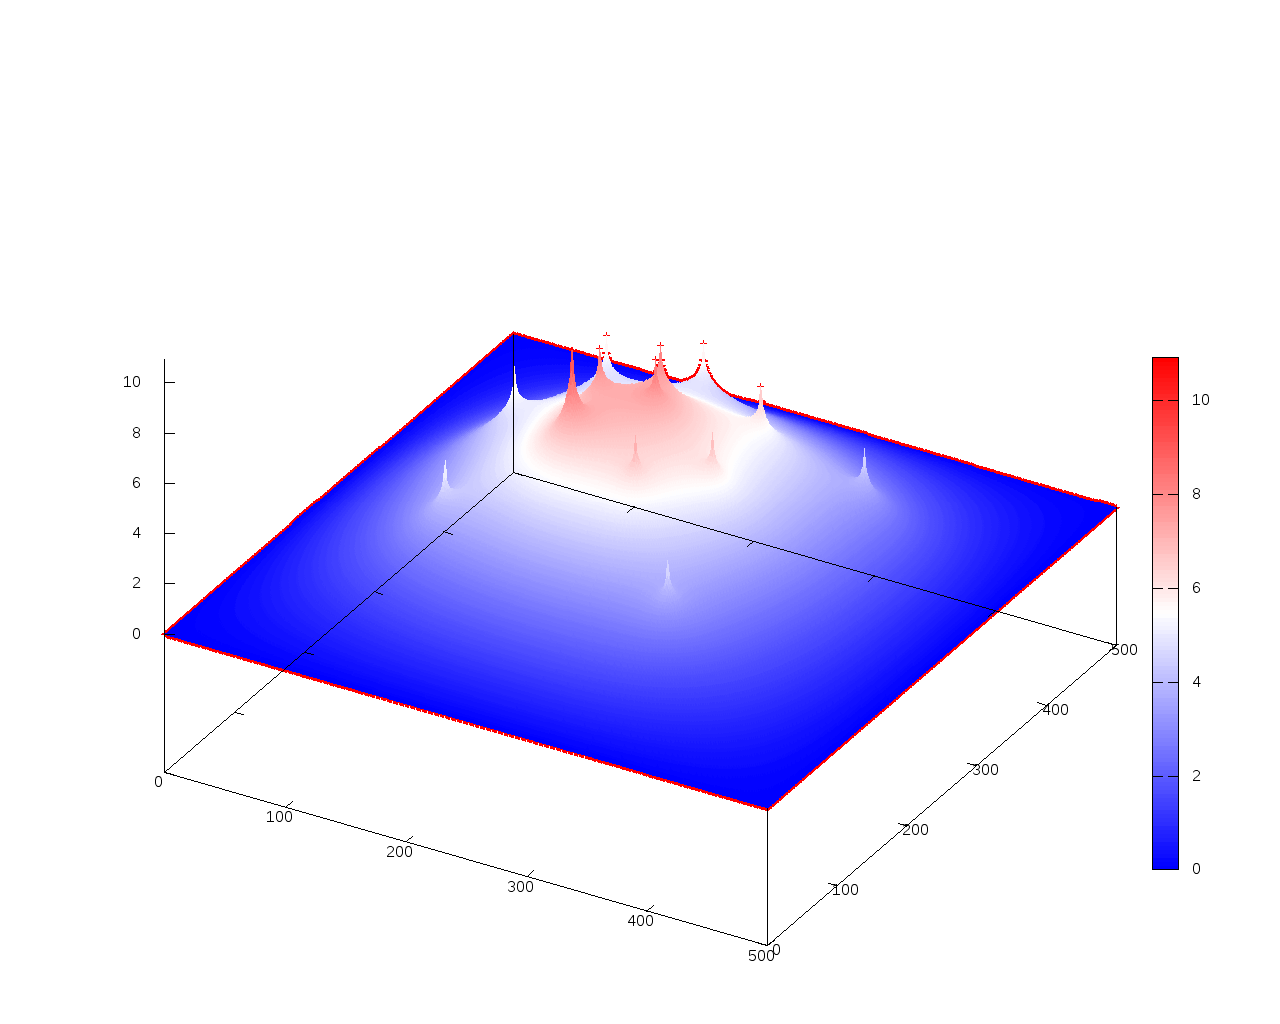
\includegraphics[width=\breite]{./images/resultate/step0144.png}
		& 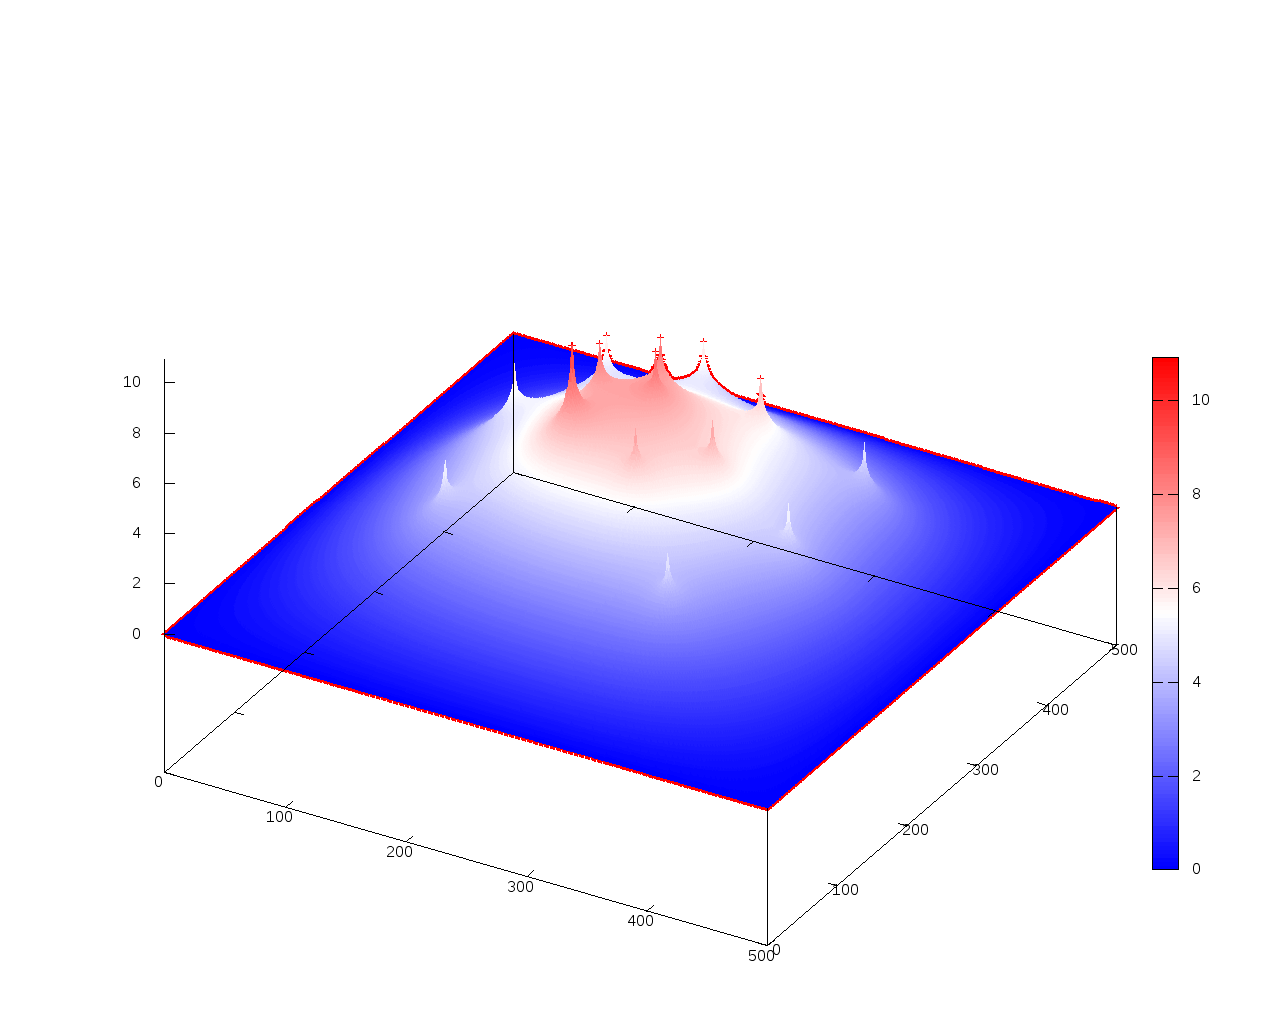
\includegraphics[width=\breite]{./images/resultate/step0149.png}\\
		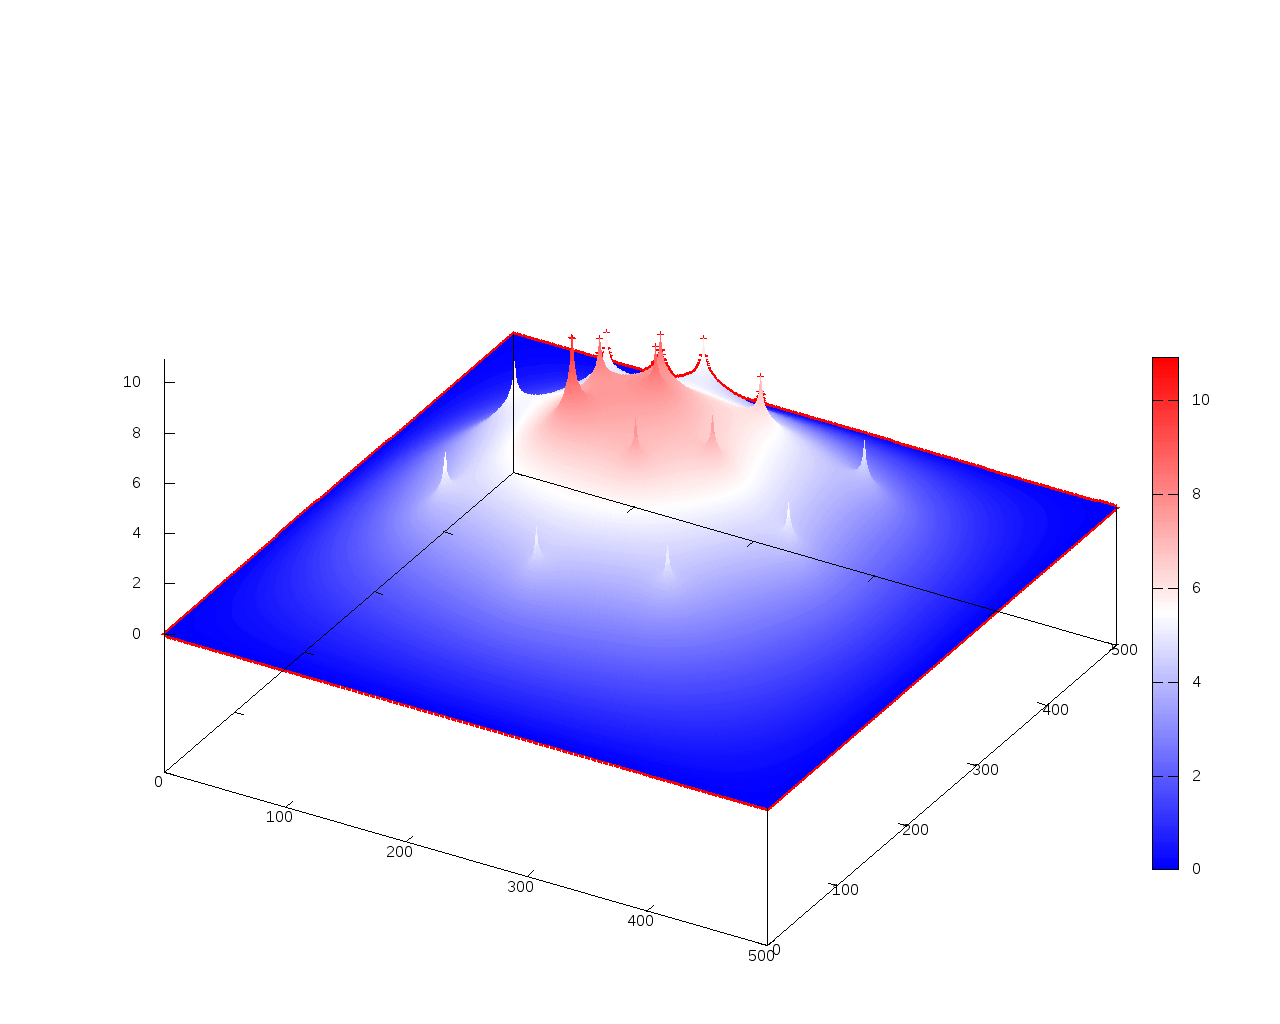
\includegraphics[width=\breite]{./images/resultate/step0162.png}
		& 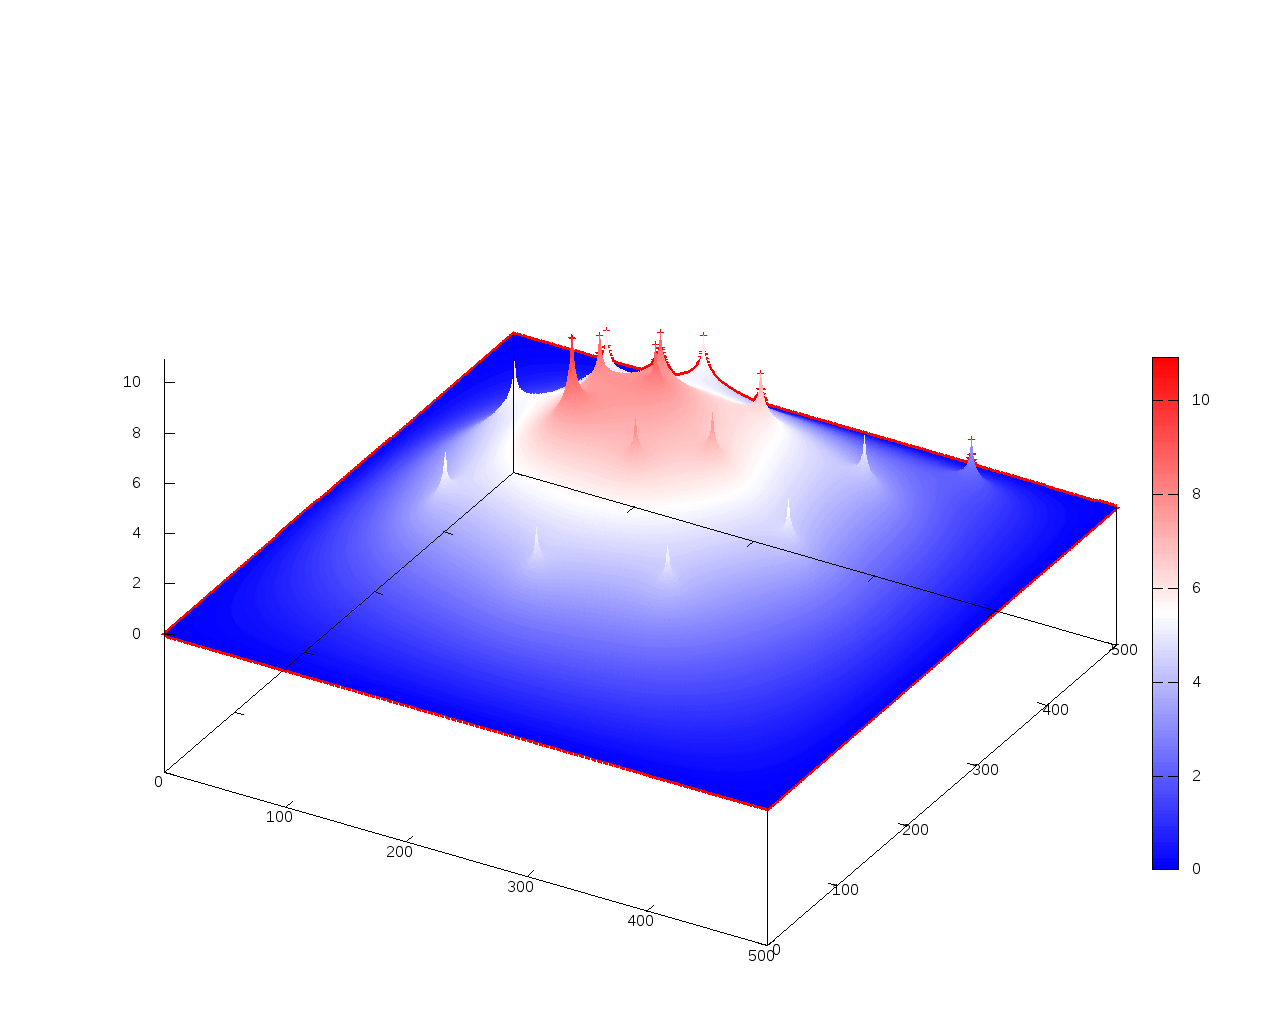
\includegraphics[width=\breite]{./images/resultate/step0175.png}
	\end{tabular}		
		\caption{Visualisierung von Green's Function: Schritte 144, 149, 162, 175 }
\end{figure}
